\documentclass{beamer}

\usetheme{Madrid}
\usecolortheme{whale}
\usepackage{xcolor}
\usepackage{etoolbox}

\usepackage{graphicx}
\usepackage{hyperref}
\usepackage[backend=biber, sorting=none]{biblatex}
\addbibresource{refs.bib}
\DeclareFieldFormat*{title}{#1}
\DeclareFieldFormat*{url}{\newline\url{#1}\nopunct}
\DeclareFieldFormat{labelnumberwidth}{#1\adddot}
\setlength{\biblabelsep}{5pt}
\renewcommand*{\bibfont}{\tiny}
\usepackage{ragged2e}

\newcommand{\biburl}[2][]{%
  \newline - \ifstrempty{#1}{}{\textcolor{cyan}{#1: }}\url{#2}\nopunct
}

% Define new counter
\newcounter{lessoncounter}

% Define new command
\newcommand{\lesson}[1]{\stepcounter{lessoncounter}\section{Lesson \arabic{lessoncounter}: #1}\subtitle{Lesson \arabic{lessoncounter}: #1}}


\title{GPT Survey: A Programmer's Perspective}
\author{Yu Zehan}
\institute{Intel FLEX}
\date{\today}

\begin{document}

\begin{frame}
  \titlepage
\end{frame}

\begin{frame}{Outline}
  \tableofcontents
\end{frame}

% \section{Lifecycle of Coding}
% \begin{frame}{Lifecycle of Coding}
%   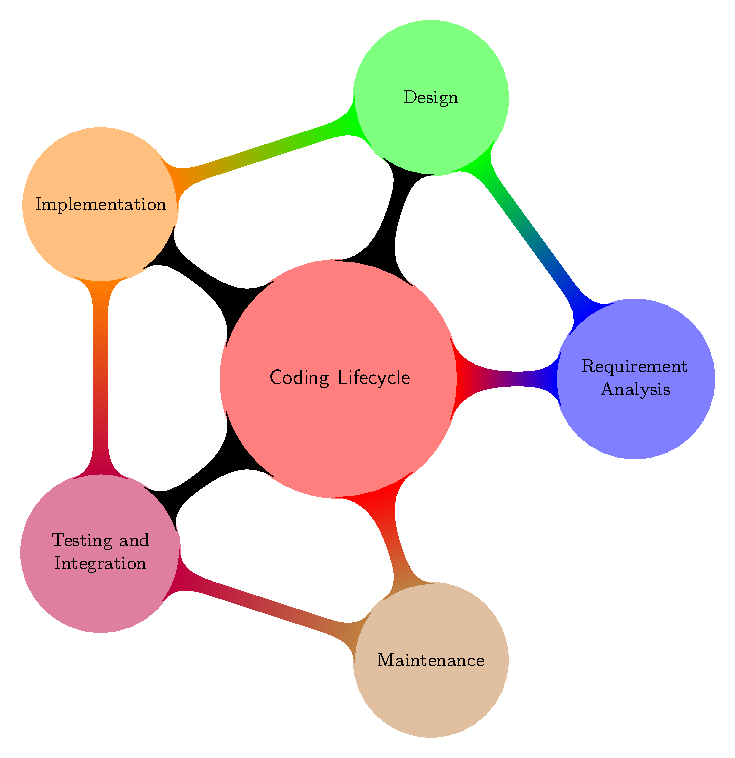
\includegraphics[width=\textwidth,height=\textheight,keepaspectratio]{tikz-code-lifecycle.pdf}
% \end{frame}


% Lesson 1
\lesson{Prompt Engineering: Principles, Techniques, and Extensions}
% 行动指南(instructions)、事实依据(facts)、思想纲领(policies)

\begin{frame}
  \titlepage
\end{frame}

% Lesson 2
\lesson{Case Studies of Coding Tasks with GPT}
\begin{frame}
  \titlepage
\end{frame}

% Lesson 3
\lesson{Integrate GPT in Whole Coding Lifecycle}
\begin{frame}
\titlepage
\end{frame}

% Lesson 4
\lesson{Cutting-Edge GPT Projects and Showcases}
\begin{frame}
  \titlepage
\end{frame}

% Lesson 5
\lesson{Customize GPT for More Power}
\begin{frame}
\titlepage
\end{frame}

\begin{frame}
\end{frame}


\section{References}
\begin{frame}[t,allowframebreaks]{References}
  \nocite{*}
  \RaggedRight
  \printbibliography
\end{frame}


\begin{frame}{FAQ}

\end{frame}

\end{document}
